\documentclass[12pt, a4paper,twoside]{tesi_upf}

%CODIFICACIÓ
\usepackage[utf8]{inputenc}


%IDIOMES
\usepackage[catalan,english]{babel}

%NOMÉS PER A OBTENIR INDICACIÓ DEL MARC EN MIDA A4
\usepackage[cam,a4,center,frame]{crop}

%PER A INCLOURE GRÀFICS I EL LOGO DE LA UPF
\usepackage{graphicx}

%FONTS TIMES O GARAMOND,
\usepackage{times}
%\usepackage{garamond}

%SENSE HEADINGS: NO MODIFICAR 
\pagestyle{plain}

%PER A L'ÍNDEX DE MATÈRIES
\usepackage{makeidx}
\makeindex

%ESTIL DE BIBLIOGRAFIA
\bibliographystyle{apalike}


%AQUEST DOCUMENT ÉS EN CATALÀ
\selectlanguage{english}

%EN COMPTES DE ÍNDEX, LA TAULA DE CONTINGUTS ES TITULA SUMARI
\addto\captionscatalan
  {\renewcommand{\contentsname}{\Large \sffamily Table of contents}}


%AFEGIU EN AQUESTA PART LES VOSTRES DADES
\title{Applying a biological model of the vestibulo-ocular reflex to control gaze stabilitzation in a humanoid robot}
\author{Xavier Duran Albareda}
\thyear{2015}
\department{Synthetic Perceptive, Emotive and Cognitive Systems group}
\supervisor{Ivan Herreros}

\begin{document}


\frontmatter


\cleardoublepage


%%%%% Dedicatòria; si no es vol posar, comenteu fins a final de dedicatòria
%\noindent To my family
%\cleardoublepage
%%%%% Final de dedicatòria

%%%%%% Agraïments; si no es vol posar, comenteu fins a final de agraïments
%\noindent {\Large \sffamily Acknowledgements}
%\cleardoublepage
%%%%%% Final dels agraïments

\vspace*{\fill}
\section*{\Large \sffamily  Abstract}

Vestibulo-ocular reflex (VOR) adaptation is one of the most studied cerebellar dependent motor learning tasks. It is used to provide insight about the connections and the coding of the circuitry of the cerebellum. Classical models used to explain motor learning with a single site of plasticity on the cerebellar cortex, but on the last decade a growing body of evidence has shown that plasticity on the brainstem is also needed for the adaptation.

The state of the art computational models of the VOR model extinction in the dark as in-phase with the vestibular information. This predicts a linear decay of the adaptation gain of the reflex, when an exponential decay has shown experimentally.

This study speculates about the existence of the nucleo-olivary inhibition (NOI), an alternative connection that would be the responsible to the extinction of the reflex that hasn't been proved yet on to exist on the physiological level. The aim is to show if the behavior of the modified model is coherent with the behavioral experiments.

\vspace*{\fill}

\cleardoublepage
%FIN DE ABSTRACTE

%PREFACI OPCIONAL. SI NO ES VOL, COMENTEU FINS EL FINAL DE PREFACI
%{\bf Prefaci}
%\cleardoublepage
%FINAL DE PREFACI

%TAULA DE CONTINGUTS: OBLIGATÒRIA
\tableofcontents

%INDEX DE FIGURES; NOMÉS ES POSA SI HI HA FIGURES
\listoffigures
%Fa que aparegui al sumari
\addcontentsline{toc}{chapter}{Índex de figures}

%INDEX DE TAULES; NOMÉS ES POSA SI HI HA TAULES
%\listoftables
%Fa que aparegui al sumari
%\addcontentsline{toc}{chapter}{Índex de taules}

\mainmatter
\chapter{Introduction}

\section{Problem statement}

NOI\cite{Herreros2013b}.

\section{State of the art}

The cerebellum has a central role in motor learning\index{motor learning}, that is the process of improving the smoothness and accuracy of movements through practice. It is not only important for learning to perform complicated movements, like playing an instrument or a sport, but also for adaptation of simple movements like reflexes along the physical changes that may occur over time.

The cerebellar cortex seems to have a uniform structure throughout the cerebellum. Its architecture is sometimes described as crystalline for it appears to be an homogeneous sheet of tissue, and is composed of repeated modules or microzones\index{microzone}, that have the same cell types that are connected in the same manner and are the functional units of the cerebellar cortex\index{cerebellar cortex}. Depending on its functional role, different microzones receive different inputs and project to different targets. A microzone along with its related subcortical structures forms what's called a microcomplex\index{microcomplex} \cite{Ito1982}, and it's considered to be a unit neuronal machine.

The uniformity on the microcircuit of the cerebellar cortex has inspired the idea that there is a single cerebellar algorithm and that different microzones process signals they receive in a similar way. The study of the cerebellum during one specific learning task may help to generalize its function to be applied to many different tasks \cite{Boyden2004}.

Vestibulo-ocular reflex\index{vestibulo-ocular reflex} (VOR) adaptation is one of the most studied cerebellar dependent motor learning tasks because of its properties: it's widespread in many species, it has well defined sensory inputs and quantifiable motor outputs, and the anatomy of circuitry is well localized \cite{Ito1982}.

\subsection{Microcircuitry of the cerebellum}

The three-neuronal pathway formed by mossy fibers, granule cells and Purkinje cells\index{purkinje cell} conforms the substrate of the multilayered computational networks of the cerebellum. Mossy fibers\index{mossy fiber} and climbing fibers\index{climbing fiber} are the inputs, and Purkinje cells are the sole output of the cerebellar cortex. As Purkinje cells project to and inhibit their target neurons in the vestibular and deep cerebellar nuclei, the entire output of the cerebellum is inhibitory.

\begin{figure}
  \centering
  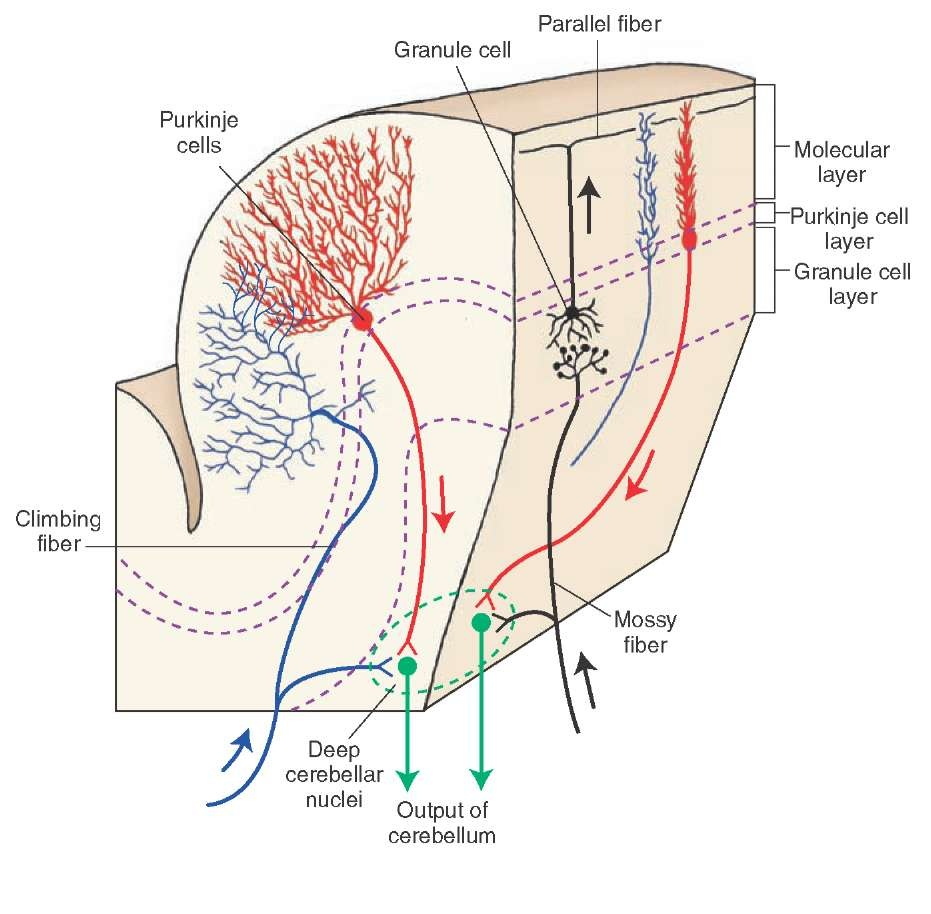
\includegraphics[scale=1]{images/circuit.jpg}
  \caption[Microcircuit of the cerebellum]{Microcircuit of the cerebellum}
\end{figure}

Mossy fibers convey information from different sources and synapse to 400 to 600 granule cells, that are the smallest and numerous neurons in the brain \cite{Marr1969}. On the contrary, granule cells integrates only a small number of mossy fibers conforming sparse coding \cite{Ito2006}. Granule cell axons bifurcate and form parallel fibers which run along the surface of the cerebellum.

Purkinje cells receive two very different types of input that have different electrophisiological effects. Parallel fibers synapse extensively on Purkinje cells and cause them to produce normal action potentials or simple spikes. Each Purkinje cell is also innervated by a single climbing fiber, arising from the inferior olive, that forms numerous synaptic contacts with the Purkinje cell dendrites. This is one of the most powerful synaptic junctions existing on the central nervous system, and every time climbing fibers fires the innervated Purkinje cell triggers a complex spike.

Parallel fibers also synapse to basket and stellate cells, the two types of interneurons of the molecular layer. They inhibit Purkinje cells and are contacted by climbing fibers. Because they are seldom differenced they are collectively called inhibitory interneurons \cite{Jorntell2010}.

\subsection{VOR adaptation task}

The flocculus, a small lobe situated on the vestibulocerebellum, is the main cerebellar region that is responsible of the control of eye movements. Its role is to optimize ocular motor performance so that the image remains still enough on the fovea so the brain is able to interpret the scene in real time \cite{Kheradmand2011}. The flocculus receives visual and vestibular information and uses it to control gaze stabilization. Vestibulo-ocular reflex, optokinetic nystagmus and smooth pursuit are under the control of the floccular region of the cerebellum.

VOR is a compensatory eye movement that stabilizes retinal images during head movements by producing an eye movement in the opposite direction, thus preventing degradation of image processing. During lifetime, changes in vestibular processing or in the mechanical properties of the oculomotor plant (as muscles develop or weaken) can cause eye-movement inaccuracies. This poor calibration results in blurred vision and VOR needs to be adapted, and the same happens when a subject starts to wear glasses. VOR produces compensatory movements in response to horizontal, vertical and translational head movements.

\begin{figure}
  \centering
  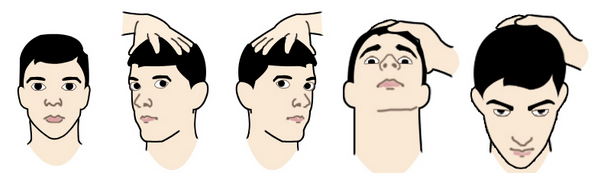
\includegraphics[scale=0.50]{images/vor.png}
  \caption[VOR reflex]{VOR reflex}
\end{figure}

In terms of control theory, VOR is a feedforward or open-loop control system since the output of the reflex has no effect on the vestibular signals input \cite{Porrill2007}, and it's controlled by an adaptive mechanism of the cerebellum. This adaptation is materialized by changing the amplitude and timing of the VOR, expressed in gain and phase values respectively \cite{DeZeeuw2005}.

In the laboratory VOR adaptation is induced in training sessions by providing visual stimuli in conflict with the vestibular stimulus. Typically screen and turntable rotation are combined to induce bidirectional gain changes in the animal VOR. Depending on the relative direction of the head and the image motion, gain and phase parameters can increase or decrease after the training periods.

An image motion in the opposite direction as the head induces
\begin{enumerate}
\item gain increase while the image in the same direction induces
\item gain decrease. In gain-decrease learning,
\item VOR cancellation happens when the speed of the head and the image are the same, and
\item phase-reversal learning when the image is faster.
\end{enumerate}

After training sessions, the performance of the VOR is measured in the dark to isolate the eye response due to head movements from that driven by visual stimuli. The persistence of the changes depends on the length of the training and the history of eye movement.

The flocculus or the entire cerebellum is not critical for generating the VOR, as it is still present in animals with the complete ablation of it, but it remains necessary for its adaptation. Lesions on the inferior olive also ended with the same result \cite{Ito2006}.

\subsection{Marr-Albus classical models}

Different models have been developed on the last forty years to explain the role of the cerebellum on motor learning tasks, most of them deriving from the classical Marr-Albus theory \cite{Marr1969,Albus1971}. The idea of the theory arises from the observation that two very different signals affect indirectly the output of the cerebellum: thousands of weak inputs from parallel fibers are integrated on the Purkinje cell to generate simple spikes; and complex spikes are provoked by the strength of a single climbing fiber synapse. The basic concept is that learning involves plasticity at the parallel fiber to Purkinje cell synapses under control of the climbing fiber that provides an error or teaching signal as in classical supervised learning paradigms. The discovery of cerebellar long-term depression (LTD) of parallel fiber synapses onto Purkinje cells \cite{Ito1982} drove to a reinterpretation of the theory where LTD was the single plasticity mechanism of cerebellar learning.

In VOR adaptation, this teaching signal is assumed to be the retinal slip, that is the motion of the visual image on the surface of the retina. When images on the retina are still then retinal slip is silent and a signal that VOR is calibrated. On the contrary, when retinal slip is present the oculomotor plant has to be compensated. This faces us with the motor-error problem: VOR adaptation, as an feed-forward system has to send motor commands to the oculomotor plant to stabilize the image on the retina. But the perfect motor commands are not known, and the error signal that arrives at the cerebellum, the retinal slip, is sensory rather than motor information.

To solve the motor-error problem, Dean and Porril define a decorrelation rule that minimizes correlations between eye movements as a predictor variable and retinal slip as a target variable \cite{Dean2002}. The cerebellum receives information from the mossy fibers that is integrated onto Purkinje cells and decorrelated from the retinal slip. The output signal from the Purkinje cells is added to the vestibular information of the head movements to produce the new motor command. Depending whether the information conveyed by mossy fibers inputs to the cerebellum is vestibular or efferent copies of the motor commands, VOR adaptation forms a recurrent or a feedback architecture \cite{Porrill2004}.

\subsection{Adaptive filter models}

The idea that the cerebellum's role in adaptation could be understood in terms of control theory led to the theory of the cerebellum as an adaptive filter. The mossy fiber signal input is analyzed in granule cells, then weighted in parallel fibers and Purkinje cells (PF-PC) synapses and finally recombined to produce the output of the filter. The adaptation consists on the bidirectional adjustment of the weights on the PF-PC, that are reduced through LTD when the parallel fiber signal is correlated with the error, and are increased through long-term potentiation (LTP) when the correlation is negative \cite{Dean2010}.

One of the predictions of the adaptive filter model that are accomplished is that most PF-PC synapses are silent. This is coherent with the idea that most of the parallel fibers are carrying signals that are irrelevant to the specific learning task, and for that they are noise. Also, the decorrelation rule needs to be able to switch between positive or negative values of the weights but the synapses are either excitatory or inhibitory. This gap can be bridged if the inhibitory interneurons pathway from granule cells to Purkinje cells are considered.

The adaptive filter model shows accurate learning on VOR adaptation when the retinal slip is not delayed. The problem is that physiological experiments show that retinal slip error signal arrives at the flocculus with a delay of 100ms. The delay causes an impairment on learning on the model at frequencies up to 10Hz achieved with an eligibility trace, but humans can perform accurately up to 25Hz \cite{Porrill2007}. This questions that cortical plasticity may be not enough for VOR adaptation task.

\subsection{Plasticity on the brainstem}

The Miles-Lisberger was an alternative model where the role of the cerebellum was not to store the motor memory but rather to compute the instructive signal, carried by Purkinje cells, guiding the induction of plasticity in the vestibular nucleus \cite{Lac1995}.

For some time the two models could explain partially physiological observations of the experimentation until a growing body of evidence due to experimental improvements showed that additional sites of plasticity appear to contribute to motor adaptation \cite{Gao2012}. Some VOR experiments with monkeys pointed to a site of synaptic plasticity not in cerebellar cortex but in the brainstem \cite{Lisberger2009}, and consensus emerged that plasticity is required for VOR adaptation both at brainstem and cerebellar cortical sites. Other studies have reported motor learning in VOR adaptation task when eliminating the climbing fiber instructive signal, suggesting that both cortical and brainstem signals produce an additive effect when both are present but neither are indispensable for motor learning \cite{Ke2009a}.

There's a question whether learning starts on the cerebellar cortex or on the brainstem. It seems that cerebellar cortex starts learning early in VOR adaptation and progressively the gain learned is transfered to the brainstem. The task of the brainstem would be to learn a simple gain to keep the cerebellar cortex plasticity free for tasks that need a quicker adaptation.

\subsection{A detailed model}

Improvements on electrophysiological recordings and on the creation of different mutant mice lines with cell-specific impairments allows to control and observe much better the contributions of the different parts of the VOR circuit. A recent and more detailed model has summed up some of the physiological and behavioral data that has been acquired during the last years \cite{Clopath2014}. This model reproduces successfully the results of a phase-reversal VOR adaptation experiment with wild-type and mutant mice \cite{Wulff2009a}.

The adaptive-filter is the initial point where plasticity on the brainstem and contribution of interneurons are added. In the model mossy fibers encode the head velocity as a sinusoidal \cite{Manuscript2009} and synapse on a network of 100 granule cells, each one distributed on different phase shifts relative to mossy fibers. Purkinje cells add up the inhibitory effect of the interneurons, that is proportional to the average activity in the granule cell network, and the excitation from the projection of granule cells on parallel fibers. The activity on the brainstem generates the motor command, and depends on the excitatory input of the mossy fibers and the inhibitory contribution of the Purkinje cells. Plasticity on the brainstem is defined by the correlation of the activity of the mossy fibers and Purkinje cells \cite{Menzies2010}, and plasticity on the PF-PC as a decorrelation rule between the vestibular information and the retinal slip \cite{Dean2002} with an added slow decay rate to the initial value of the weights.

The model shows good learning behavior with delays below 100ms as in experimentation, where models without brainstem plasticity and interneurons didn't. Clopath's detailed model may be a good baseline to work with and include further electrophysiological details available from now on.

\chapter{Methods}

\section{Research Question}

\section{Hypotheses}

\section{General Methodology Applied}

\section{Design \& Development criteria and strategies of Artifact}

\section{Experimental design and set-up}

\section{Procedures used to obtain data and results}

\chapter{Results}

\section{Data Analysis}

\section{Description of Key results obtained in the study}

\chapter{Discussion \& Conclusion}

\section{How did the results address the problem defined}

\section{What are the problems faced by the study}

\section{Validity of the results}

\section{Relevance with respect to state of the art}

\section{Future steps}

\bibliography{vor}

\backmatter
\printindex

\end{document}


%NUMERACIÓ DE LA PÀGINA EXTERIOR EXCEPTE EN LA PRIMERA PÀGINA DE CADA CAPÍTOL
\usepackage{fancyhdr}
\pagestyle{fancy}
\fancyfoot{}
\fancyfoot[RO]{\thepage}
\fancyfoot[LE]{\thepage}


%MUTIPLES ÍNDEX
%En el preàmbul
\usepackage{multind}
\makeindex{authors}
%Introducció d'entrades la forma
\index{authors}{Einstein}
%Situació de l'Índex
\printindex{authors}{Author index}
%Cal eliminar les comandes \usepakage{makeidx} \makeindex \printindex
%cal exacutar des de la línia de comandes makeindex authors
